\documentclass{article}
\usepackage[T1]{fontenc}
\usepackage{lmodern}
\usepackage{graphicx}
\usepackage{amsmath,amssymb}
\usepackage[a4paper,margin=2cm]{geometry}
\usepackage[absolute,overlay]{textpos}
\setlength{\TPHorizModule}{1mm}
\setlength{\TPVertModule}{1mm}
\usepackage[indonesian]{babel}
\usepackage{hyperref}
\setlength{\emergencystretch}{2em}
% unit: Halaman 1

\begin{document}

% === Halaman 1 (llm) ===

\begin{center}
Bahan kuliah IF4020 Kriptografi

\vspace{10mm}
\Huge \textcolor{red}{06 - One-Time Pad,}\
\Huge \textcolor{red}{Cipher yang Tidak Dapat Dipecahkan}\
\Huge \textcolor{red}{(Unbreakable Cipher)}

\vspace{136.62mm}

\vspace{10mm}
\Large Oleh: Rinaldi M

\vspace{10mm}
\large Program Studi Teknik Informatika\
Sekolah Teknik Elektro dan Informatika\
Institut Teknologi Bandung\
2026
\end{center}

% deskripsi: Foto tangan seseorang yang memegang sebuah buku kecil atau catatan berisi tabel angka-angka acak yang kemungkinan merupakan representasi dari kunci One-Time Pad.
% bbox normalisasi: [0.0600, 0.4900, 0.2300, 0.9500]
\begin{textblock*}{35.70mm}(12.60mm,145.53mm)
\noindent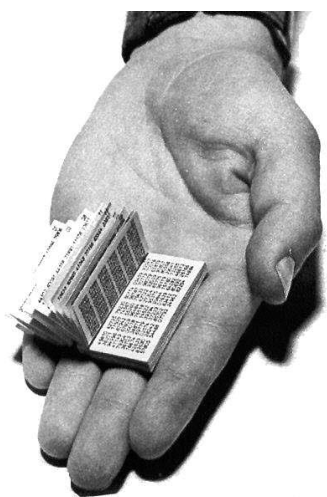
\includegraphics[width=35.70mm,height=136.62mm]{../../images/llm/page_001_img_01.png}%
\end{textblock*}

\end{document}
